\section{Problemātika un risinājuma koncepcija}
\label{s:motivation}

Šī nodaļa apraksta darba problemātiku un ieskicē izvēlētā risinājuma koncepciju. Sīkāk risinājums tiks apskatīts \ref{s:system} un \ref{s:prototype} nodaļās.

\subsection{Idejas izcelsme}

Šīs makro transformācijas sistēmas ideja ir radusies valodas Eq\footnote{Pirmkods atrodams tiešsaistē - https://github.com/zayac/eq} kompilatora izstrādes gaitā, ar ko nodarbojas zinātniskā grupa, kuras sastāvā ir cilvēki no Compiler Technology \& Computer Architecture Group, University of Hertfordshire (Hertfordshire, England), Heriot-Watt University (Edinburgh, Scotland) un Moscow Institute of Physics and Technology (Dolgoprudny, Russia). Šīs valodas sintakse bāzējas uz \LaTeX{} teksta procesora sintakses, kas ir standarts priekš zinātniskām publikācijām. Korekti uzrakstīta Eq valodas programma var tikt interpretēta ar \LaTeX{} procesoru. Perspektīvā Eq programma varēs tikt kompilēta un izpildīta uz vairākuma mūsdienīgo arhitektūru. 

Lai atvieglotu izstrādi valodā Eq tika nolemts izveidot makro sistēmu, kas ļaus pielāgot sintaksi programmētāja vajadzībām. Tomēr bez kaut kādas šablonu sistēmas makro iespējas ir ļoti ierobežotas. Tāpēc tika izlemts lietot šablonus ar minimālu regulāro izteiksmju sintaksi, kas dod brīvību sakritību aprakstīšanai. 

Kaut arī ideja un pieejas izstrāde sākās ar valodu Eq, tā tiek projektēta tā, lai varētu tikt lietota dažādām valodām, ne tikai Eq. Tas tiek darīts lai paplašināt iespējamo sistēmas pielietošanas sfēru un tās attīstības iespējas.

\subsection{Problemātika}

Valodas sintakses modificēšanai lietotāja līmenī ir izveidoti dažādi risinājumi, daži no kuri ir izskatīti \ref{s:related} nodaļā. Toties katrs no eksistējošiem risinājumiem ir kaut kādā mērā ierobežots savās iespējās. Šī nodaļa parāda projektētās transformācijas sistēmas pieeju un pamato risinājuma koncepcijas izveidi.

Viena no metodēm, kā varētu ļaut lietotājam paplašināt valodas sintaksi ir izveidot kross-kompilatoru, kas transformētu jauno sintaksi tā, lai standarta kompilators to varētu atpazīt. Toties tā kā lielākās moderno programmēšanas valodu daļas sintaksi ir grūti noparsēt lietojot automātiskus rīkus, kross-kompilatora izveidošana var būt problemātiska. Zemāk ir piedāvāti daži piemēri gadījumiem no populāras valodas C, kad automātiskā parsēšana ir neiespējama.

\begin{enumerate}
\item
Valodā C lietotājs var nodefinēt patvaļīgu tipu lietojot konstrukciju \verb|typedef|. Šāda veida iespēja padara neiespējamu šādas izteiksmes apstrādi \verb|(x) + 5|, ja vien mēs neesam pārliecināti, kas ir \verb|x| - tips vai mainīgais. Ja \verb|x| ir tips, tad šī izteiksme pārveido izteiksmes \verb|+ 5| vērtību uz tipu \verb|x|. Ja \verb|x| ir mainīgais, tad šī izteiksme nozīmē vienkāršu mainīgā \verb|x| un vērtības \verb|5| saskaitīšanu. 
\item
C valodā eksistē operators postfikss operators \verb|++|, kas palielina argumentu par vienu vienību. Pieņemsim, ka ir iespēja paplašināt C valodas sintaksi ar infiksu operatoru \verb|++|, kas savieno divus masīvus un pierakstīt konstanšu masīvus \verb|[1, 2, 3]| veidā. Tad izteiksme \verb|a ++ [1]| būtu nepārsējama, jo eksistē vismaz divi to interpretācijas veidi. Tas varētu tikt saprasts ka postfiksā operatora \verb|++| pielietošana mainīgam \verb|a| un tad \verb|a| indeksēšana ar \verb|[1]|. Vai arī tas varētu būt divu masīvu \verb|a| un \verb|[1]| konkatenācija.
\end{enumerate}

Dažreiz arī programmatūras koda dalīšana pa daļiņām ir atkarīga no šī koda konteksta, kas padara ne tikai parsēšanas procesu, bet arī leksēšanas procesu neautomatizējamu.

\begin{enumerate}
\item
Valoda C++ ļauj lietotājam izveidot ligzdveida veidnes, piemēram, šādas \verb|template <typename foo, list <int>>|. Šajā gadījumā simboli \verb|>>| aizver divas atvērtās grupas pēc kārtas. Lai tas tiešām būtu atpazīts, ka grupu aizvēršana, lekserim jāzina simbolu konteksts, vai arī jāseko valodas gramatikai, jo parasti simbolu kombinācija \verb|>>| nozīmē operāciju pārbīdei pa labi.
\item
Gadījumā, ja lietotājam ir dota iespēja definēt savus operatorus, ieviešot operatoru, kas pārklāj eksistējošos, ir jāmaina leksēšanas likumus. Piemēram, ja lietotājs definē unāru operatoru \verb|+-|, tad izteiksmei \verb|+-5| ir jābūt saprastai ka \verb|(+-, 5)|, nevis ka \verb|(+, -, 5)|.
\end{enumerate}

Apskatītie piemēri parāda to, ka automātisku parsētāju ģeneratoru lietošana dažreiz var būt tik pat sarežģīta, ka parsētāja rakstīšana ar rokām. Parsētāju ģeneratori nav piemēroti pakāpeniskām valodas sintakses evolūcijām, to izveidoto parsētāju pārģenerēšana aizņem laiku un resursus.

Izrādās, ka daudzām eksistējošām valodām parsētāji tiek rakstīti manuāli\footnote{Piemēram C/C++/ObjectiveC kompilators GNU GCC \cite{GCC}, clang kompilators LLVM \cite{clangLLVM}, JavaScript Google V8 \cite{JavascriptGoogle}}. Tas nozīmē, ka visticamāk arī kross-kompilatoru būs jāraksta manuāli, risinot eksistējošās gramatikas konfliktus, un oriģinālvalodas gramatikas izmaiņu gadījumā būs jāpastrādā abi kompilatori.

Šīs darbs izvirza pieeju, kas lietos eksistējošo valodas parsētāju par pamatu savam darbam un piedāvās likumu kopu, kas ļaus paplašināt valodas gramatiku. Taču patvaļīgas lietotāja iniciētas gramatikas izmaiņas (gramatikas likumu pievienošanas un dzēšanas) var novest pie nekontrolējamas valodas evolūcijas. Tāpēc aprakstāmā pieejā tiek piedāvātas ierobežotas izmaņu iespējas, kas tiks daļēji kontrolētas ar speciāli izveidotas tipu sistēmas palīdzību.

Projektētā sistēma ļaus ieviest jaunas konstrukcijas, konstruējot tās no jau eksistējošām valodas vienībām. Tā transformēs programmas gabalus attiecīgi pierakstītiem likumiem tā, lai valodas sākotnējā gramatika būtu tiem pielietojama. Šīs transformācijas korektumu nodrošinās tipu pārbaudes sistēma. Transformācijas korektums šī darba ietvaros nozīmē to, ka transformācijas izejas daļiņu virkne būs korekta uzrādīta transformācijas beigu tipa vienība. Piemēram, ja makro tiek uzrādīts, ka beigu transformācijas tips būs kaut kāds identifikators, bet pēc pārveidošanas no daļiņām sanāks izteiksme, šāds makro netiks akceptēts.

Ļoti līdzīgu uzdevumu, izņemot tikai transformāciju korektuma pārbaudi, pilda arī vispārējie teksta priekšprocesori. Jebkura priekšprocesora viens no galveniem mērķiem ir vienas elementu virknes aizvietošana ar citu. Virknes vienība var būt atšķirīga atkarībā no priekšprocesora, bet parasti šī vienība ir kādu vienas klases rakstzīmju kopa. Klašu daudzums parasti ir fiksēts (skaitlis, burts, tukšums, u.t.t.). Dažreiz zīmes piederība pie klases ir statiska, ka C priekšprocesorā, dažreiz ir dinamiska, ka, piemēram, \TeX{}, kur par atdalošo var definēt jebkādu simbolu. Tad apstrāde ir šo virkņu aizvietošana ar citām izveidotām virknēm.

Svarīgākā problēma šādai teksta apstrādes pieejai ir tas, ka tai neiespējams pārbaudīt rezultējošā koda korektumu sākotnējās valodas ietvaros. Apskatīsim sekojošu C makro piemēru:
\begin{verbatim}
#define foo(x, y) x y
\end{verbatim}

Pirmkārt, šādam makro nav iespējams statiski izsecināt rezultāta tipu tā ielasīšanas brīdī un izveidot kļūdas paziņojumu gadījumā, ja makro satur transformācijas, kas varētu sabojāt pārveidojamo kodu. Transformācijas rezultāta izrēķināšana ir iespējama tikai pārējā programmas teksta apstrādes laikā, jo kaut arī \verb|foo(5, 6)| tiks pārveidots par \verb|5 6|, gan \verb|foo(, 5)|, gan \verb|foo(5, )| tiks pārveidots par \verb|5|. Otrkārt, tā kā komats ir makro daļa, nav iespējams kā pirmo makro argumentu padot virkni \verb|5, 6|. To var izdarīt tikai ievietojot argumentu iekavās, tad \verb|foo((5, 6), 7)| tiks pārveidots par \verb|(5, 6) 7|.

Gadījumā, ja ir nepieciešams kaut kādā veidā saplacināt sarakstu, ir nepieciešams izveidot 2 makro, piemēram:
\begin{verbatim}
#define first(x, y) x
#define bar(x, y) first x y
\end{verbatim}

Bet aprakstītais makro strādā tikai gadījumos, kad argumentiem ir pareizs tips. Piemēram, izteiksme \verb|bar((5, 6), x)| tiks pārveidota par \verb|5 x|. Bet izteiksme \verb|bar(5, 6)| tiks pārveidota par \verb|first 5 6|, kaut arī tai vajadzētu izraisīt kļūdu. 

%Var redzēt, ka vispārīgā gadījumā nav iespējams statiski izveidot nekādus secinājumus, tā kā makro rezultāts ir atkarīgs no argumentiem, kuriem tas ir pielietots. Bet patiesībā arī nekādus dinamiskus secinājumus nav iespējams izveidot, jo apstrādājot tekstu neeksistē korektuma kritēriji.

Pat neņemot vērā grūtības mēģinot pierādīt transformācijas korektumu, teksta makro sistēmai trūkst iespēju, lai izveidot jaunas valodas konstrukcijas. Piemēram, būtu dabiski reprezentēt skaitļa moduli ar pierakstu \verb/|a|/. C priekšprocesors, savukārt, ļauj veidot tikai prefiksa formas funkciju makro un konstanšu makro. Jā arī kāda makro sistēma ļautu izveidot minēto pierakstu, parādītos problēmas gadījumos, kad vienam un tam pašam simbolam eksistē dažas nozīmes, piemēram, ar pierakstu \verb/| (a | b) |/, kam jābūt pārveidotam uz \verb/abs(a | b)/.

Apskatītie piemēri parāda, ka ne kross-kompilēšana, ne programmas teksta priekšprocesēšana vispārpieņemtā veidā neder vēlamā rezultāta sasniegšanai. Par šīs problēmas risinājumu varētu kļūt transformācijas sistēma, kas apstrādā nevis programmas tekstu, bet gan programmas daļiņu un reducēto produkciju -- pseido-daļiņu virknes. 

Lai padarītu transformācijas sistēmu vairāk spēcīgu un ļautu atpazīt vispārīgākas virknes, tās makro šabloni tiks paplašināti ar regulāro izteiksmju elementiem. Šādi šabloni ļaus meklēt plašākas sakritības joprojām saglabājot iespēju kontrolēt pārveidojumu korektumu.

Šādā sistēma dos iespēju paplašināt valodu lietotāja līmenī, nevis kompilatora līmenī. Tas arī dos lielāku brīvību izmaiņu izstrādē, jo lietotājiem būs iespēja veidot makro bibliotēkas ar jaunām iespējām un izplatīt tās. Tā varēs būt pielāgota dažādām valodām, jo tā strādās ārpus paplašināmās valodas gramatikas.

\subsection{\label{sbs:sys_approach}Sistēmas koncepcija}

Aprakstāmā transformācijas sistēma tiek projektēta ņemot vērā divu eksistējošo pieeju pieredzi. Pirmā no pieejam ir programmas koda priekšprocesēšana - koda makro ierakstu apstrāde pirms parsētāja darba sākšanos. Priekšprocesors parasti aizvieto kaut kādas konstrukcijas ar citām noteikti definētam konstrukcijām. Otrā pieeja ir adaptīvās gramatikas - gramatikas, kas ļauj programmas kodam modificēt savas valodas gramatiku. Abas pieejas dod ļoti spēcīgus rīkus programmēšanas valodu izstrādē. Tomēr abām šīm pieejām ir savas problēmas un trūkumi, no kuriem šīs sistēmas projektēšanā mēģināja izvairīties. 

Pirmā problēma, no kuras šī sistēmas izstrādē mēģināja izvairīties ir nekorekta simbolu ar divām nozīmēm apstrāde. Pieņemsim, ka mēs gribam funkciju \verb|abs(x)| apzīmēt ka \verb/|x|/. Apskatīsim izteiksmi \verb/|(a | b) + c|/, kurai vajadzētu tikt pārveidotai par \verb/abs((a | b) + c)/. Gadījumā, ja transformācijas sistēma apstrādātu vienīgi tekstu, tā nebūtu spējīga pārveidot šādu konstrukciju. Tiks apstrādāti pirmie divi \verb/|/simboli, no \verb/| (a |/, izveidojot nekorektu konstrukciju \verb/abs((a) b) + c) |/. Šīs problēmas izvēlētais risinājums ir aprakstīts \ref{sbsbs:sys_texttransform} apakšnodaļā.

Otrā problēma ir neiespējamība vispārīgā gadījumā kontrolēt dinamiskas gramatikas izmaiņas. Dinamiskas gramatikas ir ļoti spēcīgs rīks, kas mūsdienās gandrīz netiek lietots tādēļ, ka dodot iespēju lietotājam patvaļīgi pievienot un dzēst gramatikas likumus, tiek zaudēta iespēja kontrolēt izmaiņu korektumu. Robežgadījums varētu būt tad, kad sākotnējā gramatika tiek pilnībā aizvietota ar citu gramatiku. Tad, kaut arī sākotnējā gramatika bija derīga parsēšanai ar eksistējošo algoritmu, jaunai gramatikai var piemīt īpašības, kas neļaus to apstrādāt (piemēram, kreisā rekursija LL parsētāju gadījumā). Šīs problēmas izvēlētais risinājums ir apskatīts \ref{sbsbs:sys_dynamicgrammars} apakšnodaļā.

Trešā problēma ir tas, ka nav iespējams vienkārši ieviest gramatikas modifikācijas jau eksistējošā valodas parsētāja, ja vien tā arhitektūra no sākuma atbalsta gramatikas izmaiņas. Bet tā kā parasti šāda iespēja netiek iekļauta, visticamāk būs nepieciešamas nopietnas parsētāja adaptācijas. Aprakstāmā sistēma, savukārt, mēģina dot iespēju paplašināt valodas gramatiku bāzējoties uz vienu no plaši lietojamam parsētāju arhitektūrām. Kā tas tiks darīts ir aprakstīts  \ref{sbsbs:sys_parsermodifications} apakšnodaļā.

\subsubsection{\label{sbsbs:sys_texttransform}Teksta pārveidošana}

Ir dažādas pieejas programmu pirmkoda priekšprocesēšanai. Visvairāk izplatītas no tām ir divas pieejas. Viena no pieejām ir sintaktiskā pieeja - sintaktiskie priekšprocesori tiek palaisti pēc parsētāja darbības un apstrādā abstraktos sintaktiskos kokus (AST), ko tas ir uzbūvējis. Šāda tipa priekšprocesori netiks apskatīti šajā darbā, jo to darbībai ir nepieciešams korekts sintakses koks. Aprakstāmās sistēmas gadījumā sintakses koka uzbūvēšana var būt neiespējama tad, kad gramatikā tika ieviestas kaut kādas jaunas konstrukcijas. Sistēmai jānostrādā pirms sintaktiskā koka izveidošanas. Otra no priekšprocesēšanas pieejām ir leksiskā. Leksiskie priekšprocesori tiek palaisti pirms pirmkoda parsēšanas un tiem nav zināšanu par apstrādājamas valodas sintaksi (piem. C/C++ priekšprocesors).

Leksiskie priekšprocesori pēc savām īpašībām ir tuvi aprakstāmai sistēmai. Ar makro valodu palīdzību tiem tiek uzdoti koda pārrakstīšanas likumi, un kods tiek pārveidots attiecīgi tām. Bet leksisko priekšprocesoru vislielākais trūkums ir tas, ka tie apstrādā tekstu pa simboliem neievērojot izteiksmju un konstrukciju struktūru. Apskatīsim jau minētu piemēru \verb/abs((a | b) + c)/. Ar tādu makro sistēmu, kas neievēro koda struktūru, tātad neievēro to, ka patiesībā \verb/(a | b) + c/ ir atomāra konstrukcija izteiksmē, šādu koda gabalu pareizi apstrādāt nevarēs\footnote{C/C++ priekšprocesors vispār neatļaus tādu konstrukciju izveidot, kaut arī šāds pieraksts ir diezgan loģisks no matemātiķu skatu punkta. C/C++ makro sistēma ļauj veidot tikai makro konstantes un prefiksa formas funkcijas.}.

Priekšprocesoru var iemācīt apstrādāt šāda veida konstrukcijas un atpazīt tos, ka atomārās izteiksmes. Bet tas nozīmēs, ka priekšprocesoram būs jāzina apstrādājamas valodas gramatika, tātad nozīmē ka būs divreiz jāimplementē sintakses atpazīšana.

Lai izvairīties no šīs problēmas tika izvēlēts apstrādāt nevis programmas tekstu, bet gan programmas daļiņu un reducēto produkciju -- pseido-daļiņu -- virkni, ko daļēji jau apstrādāja parsētājs. Tas nozīmē, ka makro šablonu sintakse būs bāzēta uz daļiņu aprakstiem, nevis uz tekstuālām izteiksmēm. Piemēram, ja ir nepieciešams izveidot šablonu, kas pārveidos funkcijas ar nosaukumu \verb|bar| par funkcijām ar nosaukumu \verb|foo|, makro šablonā būs jāieraksta daļiņa ar tipu \verb|id| un vērtību \verb|bar| - \verb|{id:bar}|. Tad, kad programmas daļiņu virknē tiks atrasta daļiņa ar šādu tipu un vērtību, tā tiks aizvietota ar daļiņu \verb|{id:foo}|. Šāda pieeja dod iespēju programmas tekstā meklēt specifiskus daļiņu tipus, nevis specifiskas teksta daļas. Tas dod iespēju meklēt, piemēram, jebkādus identifikatorus, šablonā norādot daļiņu \verb|{id}| bez vērtības. 

Makro šablonu sistēma arī ļauj lietot pseido-daļiņas savu šablonu aprakstos, t.i. ļauj lietot daļiņu \verb|{expr}|. Pseido-daļiņa \verb|{expr}| dotajā sintaksē apzīmē kādu izteiksmi. Tā tiek saukta par pseido-daļiņu tādēļ, ka programmas tekstā tā ir reprezentēta ar citu daļiņu virkni, kas tiek aizvietota gramatikas likuma reducēšanas brīdī. Patiesībā tā ir atomāra vienība.

Tā kā aprakstāmā sistēma tiek izstrādāta tā, lai tā varētu darboties zinot pēc iespējas mazāk par valodas gramatiku, tā nezina, kādas varētu būt izteiksmes dotajā valodā. Tad, kad transformācijas sistēmu makro ir atrodama šāda pseido-daļiņa, sistēma nemēģina pati izsecināt, vai šāda daļiņa ir nolasāma no parsētās virknes. Lietojot speciālu saskarni tā "pajautā" parsētājam, vai sagaidītā pseido-daļiņa ir atrodama sākot no dotās daļiņas virknē. Gadījumā, ja parsētājs var izveidot izteiksmi, tas paziņo par to, un transformācijas sistēma turpina virknes apstrādi. Piemēram, konstrukciju \verb/(a | b) + c/ parsētājs atpazīs ka pseido-daļiņu \verb|{expr}|.

Gadījumā, ja kāds no šabloniem tiks atpazīts ieejas virknē, atpazītā apakšvirkne tiks pārveidota citā, kas aizvietos atrasto. Tālāk aizvietotā virkne tiks apstrādāta ar sākotnējo valodas gramatiku.

Otrā leksiskā tipa priekšprocesoru problēma ir tas, ka tie strādā ārpus programmas tvērumiem. Tas nozīmē, ka tvēruma sākuma daļiņa (piemēram, figūriekava, C/C++, Java un citu valodu gadījumā) tiek uzskatīta par parastu tekstu un var tikt pārrakstīta. Loģiskāk būtu, ja konkrētā tvērumā definēti makro tiktu mantoti līdzīgi ka mainīgie, kas nozīmē, ka šabloni, kas ir specifiski tvērumam, būtu ar lielāku prioritāti ka tie, kas definēti vispārīgākā tvērumā. 

Sistēmas sakrišanas meklēšanas mehānisms tiks izstrādāts ņemot vērā programmas tvēruma maiņu. Tātad šabloni, kuri tiek ieviesti konkrētā tvērumā, strādās tikai tā ietvaros. Pēc izejas no tvēruma ielasītie makro tiek aizmirsti un tālāk sistēma strādā bez tiem.

\subsubsection{\label{sbsbs:sys_dynamicgrammars}Dinamiskas gramatikas}

Ir dažādas iespējas lietot dinamiskas gramatikas. Viena no tām ir pieeja, kas ļauj kontrolēt tā saukto programmas statisko semantiku. Par statisko semantiku dažādos rakstos sauc kontekst-atkarīgu sintaksi, piemēram, attiecību starp mainīgā deklarāciju un tā lietošanas ierobežojumiem. Otra pieeja ļauj pa tiešo pievienot un dzēst valodas gramatikas likumus. Tā kā aprakstāmā sistēma nav piemērota statiskai tipu pārbaudei, bet gan tiek veidota lai varētu paplašināt eksistējošo sintaksi, tā pēc būtības ir tuvāka otrai dinamisko gramatiku lietošanas pieejai.

Transformācijas sistēma neļaus pievienot un dzēst apstrādātās valodas gramatikas likumus. Toties tā ļaus pievienot jaunas konstrukcijas pievienojot likumus makro sistēmas kopai. Katrs makro pievieno jaunu daļiņu virknes pārrakstīšanas likumu, kas tiek izpildīts, kad tiek atrasta sakrišana ar makro specificētu šablonu. Tātad jaunās konstrukcijas daļiņu virknē ir atpazītas un pārrakstītas uz konstrukcijām, kuras jau ir zināmas parsētājam.

Lai nodrošinātu gramatikas likumu pievienošanas kontroli, tiek ieviestas dažas tipu specifikācijas. Katrs no makro attiecas uz kādu konkrētu gramatikas produkciju, un nevar tikt pārbaudīts citā parsēšanas brīdī. Katram makro pārrakstīšanas likumam arī ir specificēts tips, kas tiek lietots lai statiski pārliecināties par to, ka transformācija ir korekta dotā tipa ietvaros. Tipu sistēma detalizētāk ir aprakstīta \ref{sbsbs:sys_typesystem} apakšnodaļā.

\subsubsection{\label{sbsbs:sys_parsermodifications}Parsētāja modifikācijas}

Vēl viena svarīga dinamisku gramatiku īpašība ir tas, ka to lietošanai ir nepieciešams speciāli izstrādāts parsētājs, kas atļauj savu parsēšanas tabulu modifikācijas. Ir jāeksistē iespējai pievienot un dzēst attiecīgus gramatikas likumus, kā arī parsētājam jāprot pārbūvēt parsēšanas tabulas atbilstoši ieviestām izmaiņām.

Šī dinamisku gramatiku īpašība ļoti ierobežo iespēju lietot tos jau eksistējošo valodu paplašināšanai. Šāda veida papildināšana vairākumā gadījumu nozīmēs jauna parsētāja izveidošanu. Bet zinot, ka mūsdienīgām valodām parasti eksistē vairāki kompilatori, kurus izstrādā dažādi cilvēki, šādu izmaiņu ieviešana globālajā līmenī var kļūt neiespējama.

Aprakstāmā sistēma, savukārt, ir domāta ka palīgrīks parsētājam. Parsētāju izmaiņas, kas būs nepieciešamas integrēšanai ar sistēmu ir minimālas. Tas dos iespēju lietot to jebkuram parsētājam, kas atbilst dažiem apstrādes nosacījumiem, kas ir apskatīti \ref{sbs:sys_parserqualities} apakšnodaļā.

Sistēma dos iespēju papildināt valodas sintaksi bez nepieciešamības pilnībā pārstrādāt valodas parsētājus. Tā strādās ārpus valodas gramatikas. Pirms vai pēc katras produkcijas apstrādes ar standartu valodas gramatiku likumiem tiek izsaukta transformācijas sistēma. 

\subsection{Sistēmas vieta kompilēšanas procesā}

Šī nodaļa vienkāršoti apskata kā parasti notiek programmu kompilēšanas process un iezīmē procesā vietu priekš transformācijas sistēmas.

Parasti kompilēšanas process sastāv no diviem posmiem, no analīzes un no sintēzes. Analīzes posmā programma tiek sadalīta sastāvdaļās un no šīm daļām tiek veidota programmas struktūra. Šī struktūra tiek lietota lai izveidot starpfāzes reprezentāciju programmai - abstrakto sintakses koku (ASK). Analīzes fāzē var tikt atrastas sintaktiskas vai semantiskas izejas koda kļūdas un kompilēšanas process var tikt pārtraukts. Sintēzes posmā, savukārt, no ASK un papildus informācijas par programmas datiem, kompilators veido izpildāmo kodu.

Šeit netiks apskatīts izpildāmā koda veidošanas process, jo aprakstāmā sistēma iekļaujas parsēšanas gaitā. Tomēr vajag atzīmēt, ka koda ģeneratoram ir nepieciešams korekts sintakses koks, tātad tam ir ļoti stingri definēta saskarne. Visām izejas koda pārveidošanām, jā vien tās tiek ieviestas, ir jāstrādā tā, lai analīzes fāzē izveidotais ASK būtu korekts koda ģeneratora ieejas koks.

Parasti analīzes process notiek sekojoši (sk. \ref{fig:usual_compiling} attēlu). Izejas programmas teksts tiek apstrādāts ar priekšprocesoru, kas aizvieto vienus izejas teksta gabalus ar citiem, kas tika tam definēti. Tad pārveidotais kods tiek apstrādāts ar lekseru, kas sadala programmas tekstu jēdzīgās sastāvdaļās - daļiņās. Tālāk parsētājs transformē daļiņu virkni atbilstoši valodas gramatikai izveidojot ASK.

\begin{figure}[H]
  \centering
    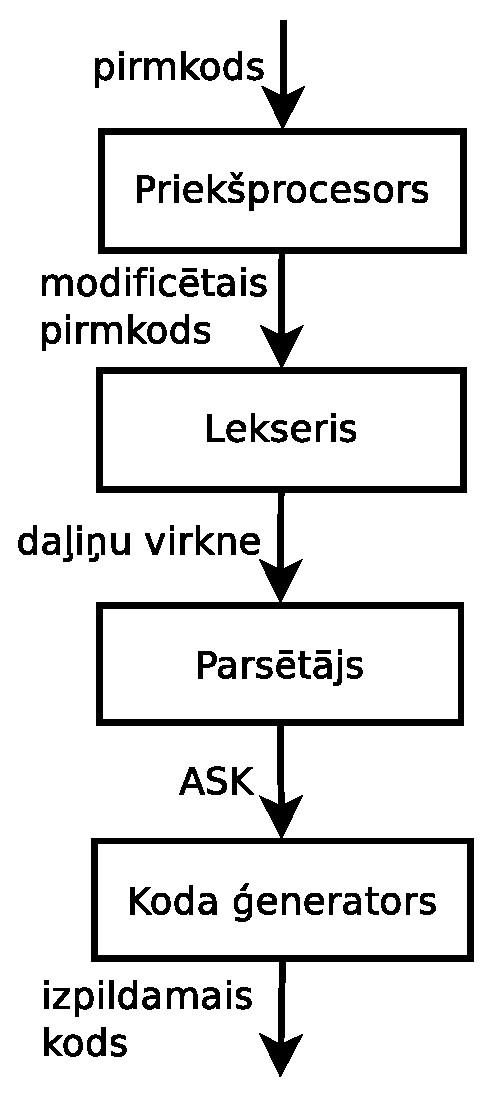
\includegraphics[scale=0.4]{pictures/usual_compiling}
  \caption{\label{fig:usual_compiling}Kompilācijas process}
\end{figure}

Transformācijas sistēma tiek veidota tā, lai tā apstrādātu daļiņu virknes paralēli ar parsētāju (sk. \ref{fig:ransform_compiling} attēlu). Tās funkcijas tiks izsauktas pirms vai pēc parsētāja produkcijas reducēšanas. Ja transformācija tiks izsaukta pirms parsētāja darbības, tad transformācijas likumiem lielāka prioritāte nekā standartiem produkcijas reducēšanas likumiem, piem. būs iespēja pārdefinēt izteiksmes \verb|a+b| uzvedību ar transformācijas palīdzību. Ja transformācija tiks izsaukta pēc parsētāja darbības, tas nozīmēs, ka nekāds standarta parsēšanas likums nav piemērots dotās virknes apstrādei un ir nepieciešamas modifikācijas. Transformācijas sistēmas uzvedības nav atkarīga no izvēlētās pieejas.

\begin{figure}[H]
  \centering
    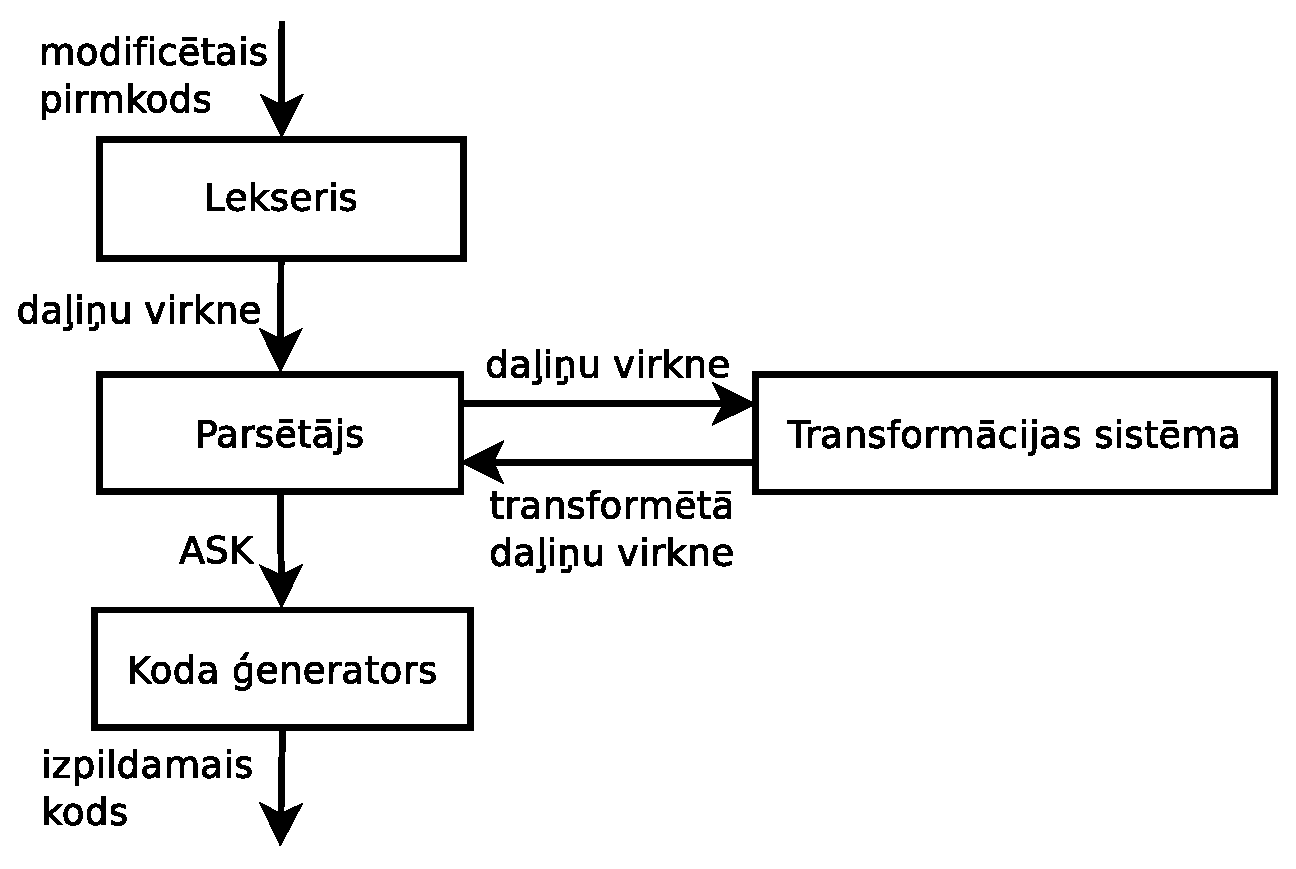
\includegraphics[scale=0.4]{pictures/transform_compiling}
  \caption{\label{fig:ransform_compiling}Kompilācijas process ar iekļauto transformācijas sistēmu}
\end{figure}

Zemāk ir parādīti makro ielasīšanas soļi, kas notiek, kad parsētājs sastopas ar makro ierakstu programmas pirmkodā:
\begin{enumerate}
\item
Parsētājs atpazīst makro sākšanos un izsauc transformācijas sistēmu.
\item
Transformācijas sistēma ielasa makro.
\item
Tipu apakšsistēma pārbauda makro tipu korektumu. Ja tipi ir korekti, turpina uz \ref{i:read_ok} soli. Ja ielasītā makro tipi nav korekti, turpina uz \ref{i:read_notok} soli.
\item \label{i:read_ok}
Transformācijas sistēma saglabā makro priekš specifiskas produkcijas, lai tālāk apstrādāt programmu.
\item \label{i:read_notok}
Transformācijas sistēma parāda kļūdas paziņojumu par to, ka ielasītā makro tips nesakrīt ar iezīmēto tipu.
\end{enumerate}

Makro atpazīšanas soļi, gadījumā, jā transformācijas sistēma tiek izsaukta pirms parsētāja mēģinājuma apstrādāt produkciju:
\begin{enumerate}
\item
Parsētājs ienāk kādā no produkciju atpazīšanas funkcijām un izsauc transformācijas sistēmu.
\item
Ja transformācijas sistēmā eksistē makro priekš dotas produkcijas, tā sāk makro atpazīšanas procesu ar \ref{i:match_start} soli. Citādi tā nedara neko un parsētājs turpina darbu ar \ref{i:match_notok} soli.
\begin{enumerate}
\item \label{i:match_start}
Transformāciju sistēma pārbauda, vai tajā vietā daļiņu virknē, uz kuru rāda parsētājs, ir sekvence no daļiņām, kas atbilst kādam no makro šabloniem. Ja šāda sekvence eksistē, turpina uz \ref{i:match_ok} soli. Ja šādas sekvences nav, turpina uz \ref{i:match_notok} soli.
\item \label{i:match_ok}
Ielasītā sekvence tiek transformēta attiecīgi makro likumam.
\item
Ielasītā sekvence daļiņu virknē tiek aizvietota ar transformēto sekvenci un parsētāja pozīcija tiek uzstādīta uz aizvietotās virknes sākumu. Transformācijas sistēma sāk darbu atkal no \ref{i:match_start} soļa.
\end{enumerate}
\item \label{i:match_notok}
Parsētājs atjauno darbu no tās pašas vietas daļiņu virknē un sāk gramatikas produkcijas atpazīšanu. %Ja produkcija ir atpazīta, parsētājs turpina darbu no soļa~\ref{i:match_first} ar nākamo produkciju. Ja produkcija nav atpazīta un daļiņu virkne ir beigusies, parsētājs apstājas. Ja produkcija nav atpazīta, parsētājs parāda kļūdas paziņojumu.
\end{enumerate}

\ref{fig:match_algorithm} attēls parāda transformācijas sistēmas palaišanu un darbību virkni diagrammas veidā.

\begin{figure}[h!]
  \centering
    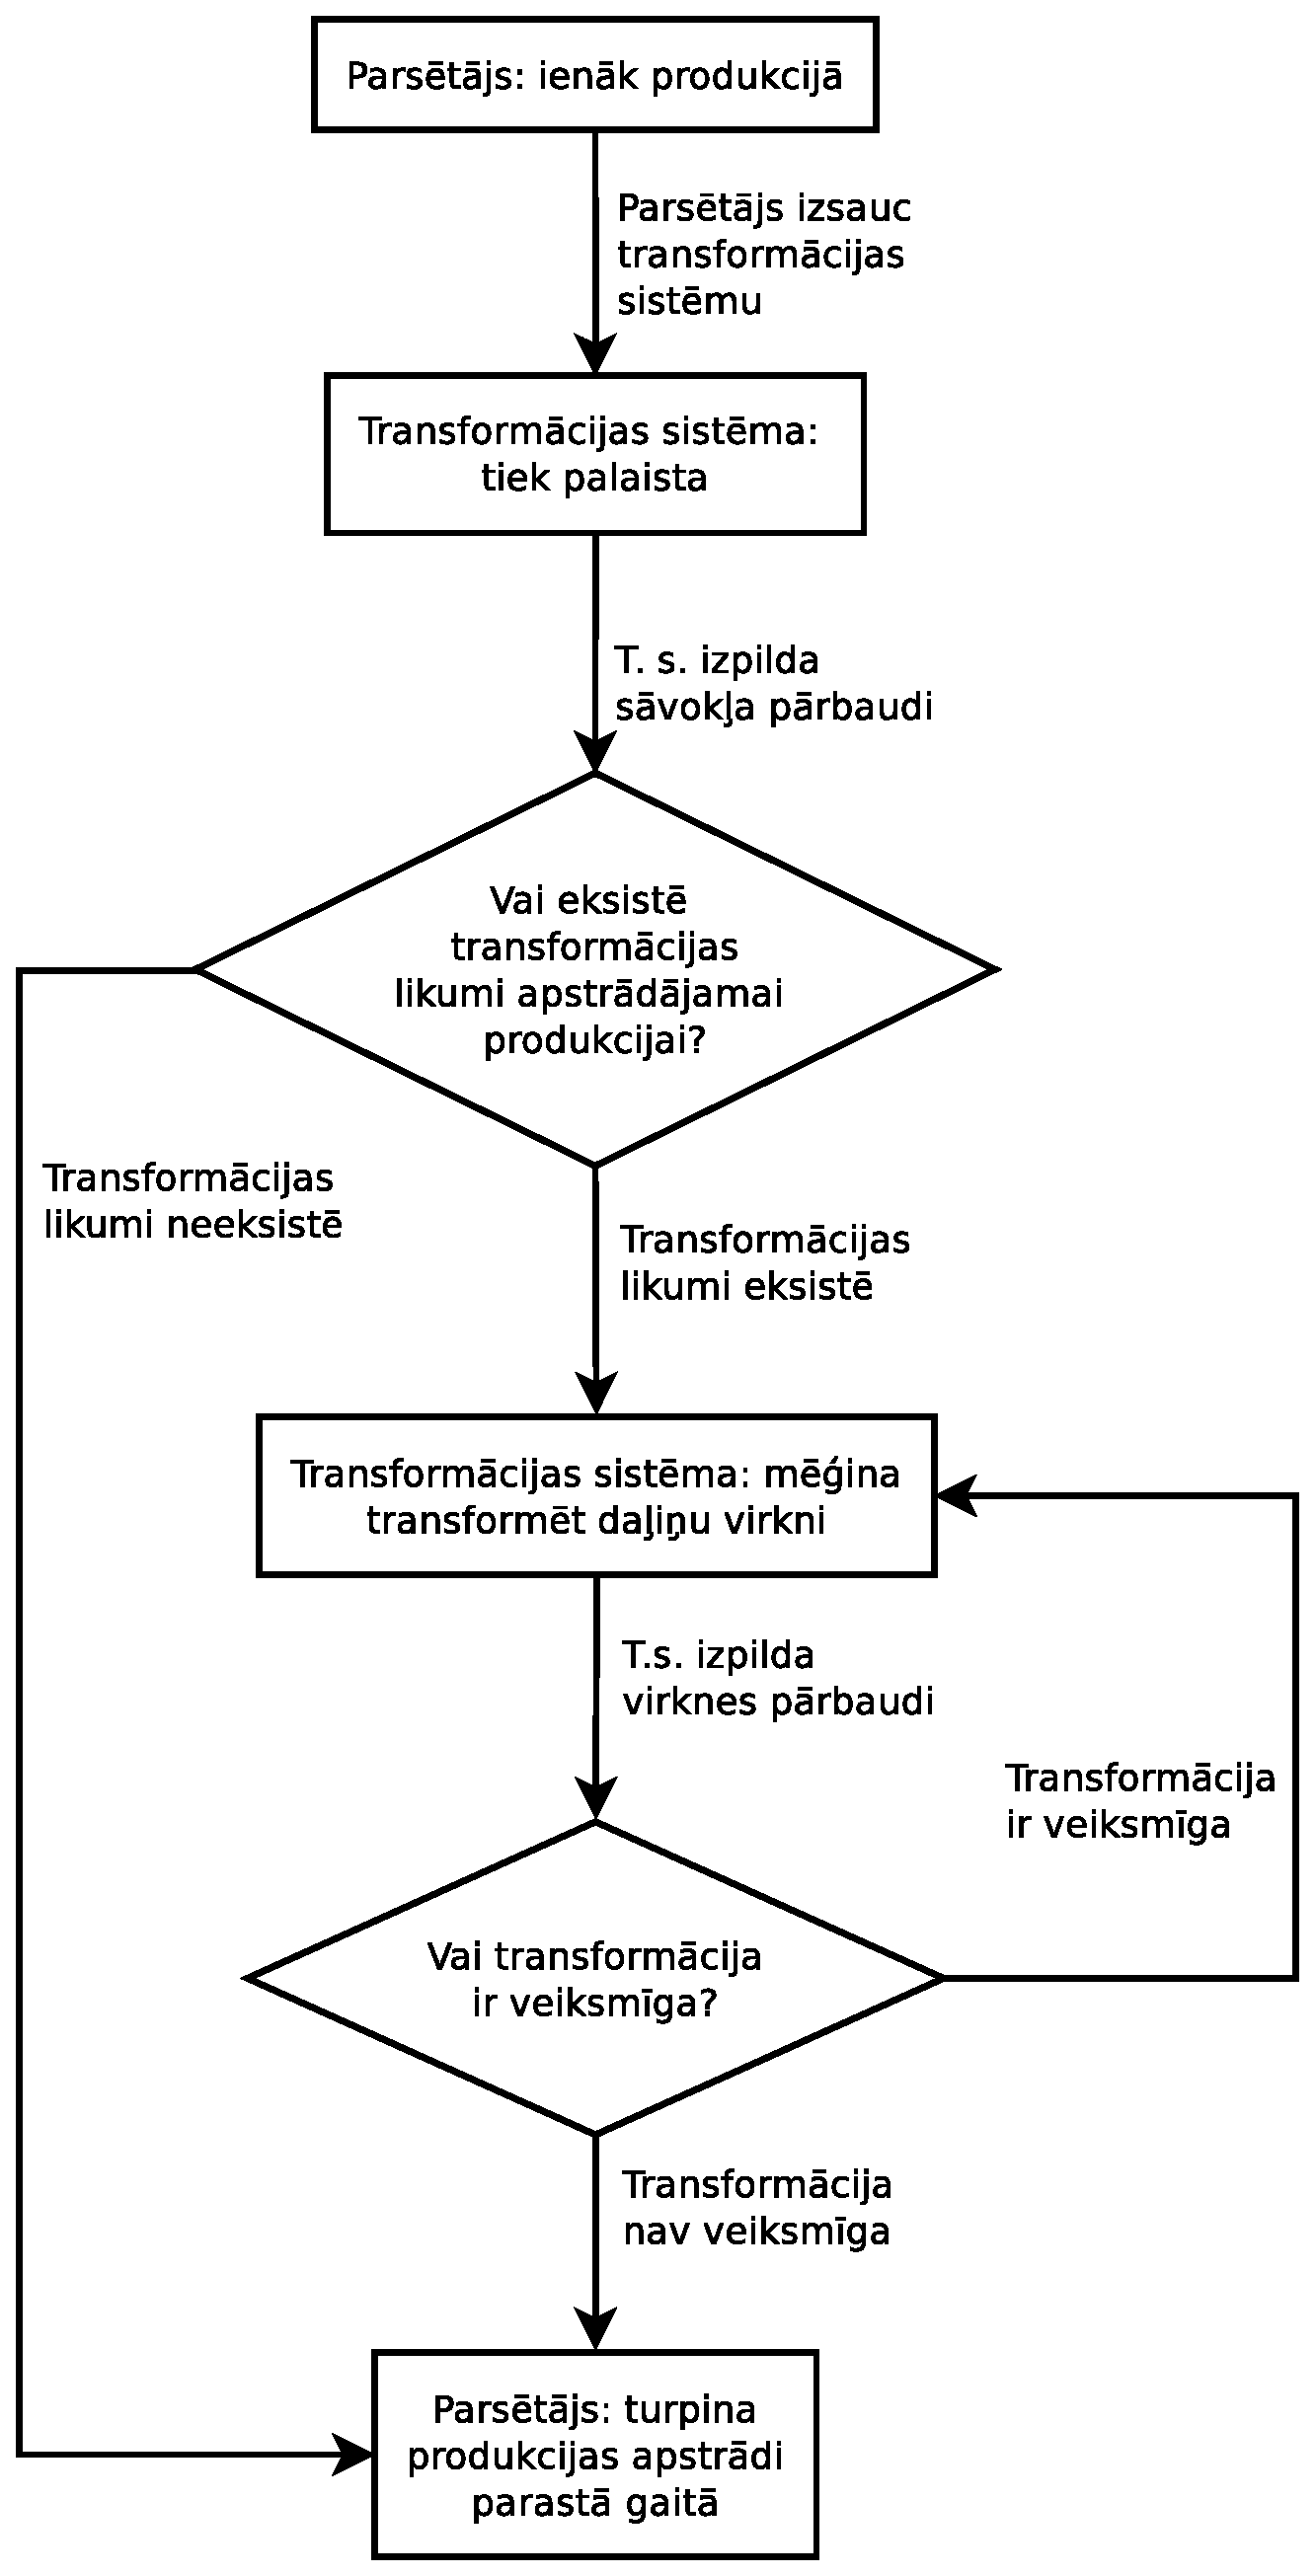
\includegraphics[scale=0.4]{pictures/match_algorithm}
  \caption{\label{fig:match_algorithm}Parsēšanas darba gaita ar iekļauto transformācijas sistēmu}
\end{figure}